\section{Risultati Sperimentali}
\label{sec:Risultati}

In questo capitolo vengono presentati e discussi i risultati ottenuti dall'implementazione dell'algoritmo \emph{Tabu Search} descritto nei capitoli precedenti. Per valutare il comportamento dell’algoritmo, si sono condotti test su diverse istanze del problema, variando i parametri chiave come \emph{tabuTenure}, \emph{maxNoImprovement} e la dimensione dei grafi.

\subsection{Setup Sperimentale}

Le prove sono state eseguite su una macchina con le seguenti specifiche:
\begin{itemize}
    \item \textbf{CPU:} Intel Core i7-1065G7 (1.30\,GHz)
    \item \textbf{RAM:} 16\,GB
    \item \textbf{Sistema Operativo:} WSL Ubuntu 20.04 (64 bit)
    \item \textbf{Linguaggio:} Java (OpenJDK 17)
\end{itemize}

Le istanze di test comprendono grafi con numero di nodi (\(n\)) variabile tra 20 e 800, e numero di archi (\(m\)) tra 60 e 10000. I pesi dei nodi sono interi positivi.

\subsection{Confronto tra Diverse Configurazioni di Parametri}

Per capire come i parametri influenzino le prestazioni, sono state confrontate diverse configurazioni di \emph{tabuTenure} (5, 7), \emph{maxNoImprovement} (10, 20, 30) e \emph{maxIterations} (500, 1000, 2000). In ciascun caso, l'algoritmo è stato eseguito 5 volte su ogni istanza, per ridurre la variabilità stocastica. A titolo di esempio, la tabella~\ref{tab:risultati1} riporta i risultati medi su un insieme di 3 istanze (piccola, media e grande).

\begin{table}[h!]
\centering
\caption{Risultati medi (5 run) per diverse configurazioni di \emph{maxIterations}, \emph{tabuTenure} e \emph{maxNoImprovement}.}
\label{tab:risultati1}
\begin{tabular}{l|c|c|c|c|c|c}
\hline
\textbf{Config.} & \textbf{Nodes} & \textbf{Arcs} & \textbf{maxIter.} & \textbf{tabuTenure} & \textbf{maxNoImpr.} & \textbf{Time (s)} \\
\hline
C1 & 20 & 60 & 500 & 5 & 10 & 0.0092 \\
C2 & 100 & 500 & 500 & 5 & 10 & 0.0608 \\
C3 & 800 & 10000 & 500 & 5 & 10 & 6.1008 \\
C4 & 20 & 60 & 500 & 7 & 20 & 0.0148 \\
C5 & 100 & 500 & 500 & 7 & 20 & 0.108\\
C6 & 800 & 10000 & 500 & 7 & 20 & 6.7292 \\
C7 & 20 & 60 & 1000 & 5 & 20 & 0.0156 \\
C8 & 100 & 500 & 1000 & 5 & 20 & 0.0836 \\
C9 & 800 & 10000 & 1000 & 5 & 20 & 6.7994 \\
C10 & 20 & 60 & 1000 & 10 & 30 & 0.021 \\
C11 & 100 & 500 & 1000 & 10 & 30 & 0.0818 \\
C12 & 800 & 10000 & 1000 & 10 & 30 & 7.2512 \\
C13 & 20 & 60 & 2000 & 7 & 10 & 0.0134 \\
C14 & 100 & 500 & 2000 & 7 & 10 & 0.062 \\
C15 & 800 & 10000 & 2000 & 7 & 10 & 6.856 \\
C16 & 20 & 60 & 2000 & 10 & 20 & 0.0168 \\
C17 & 100 & 500 & 2000 & 10 & 20 & 0.0926 \\
C18 & 800 & 10000 & 2000 & 10 & 20 & 7.54 \\
\hline
\end{tabular}
\end{table}

\noindent
Dall’osservazione dei dati in tabella~\ref{tab:risultati1} emergono due punti essenziali:
\begin{itemize}
    \item \textbf{Dimensioni del grafo come fattore dominante:}
    passando da \((20,60)\) a \((800,10000)\) nodi/archi, si registra un salto netto dei tempi di esecuzione (dell’ordine di microsecondi-millisecondi a svariati secondi).

    \item \textbf{\emph{maxNoImprovement} come parametro più incisivo:}
    a parità di \emph{maxIterations} e \emph{tabuTenure}, valori minori di \emph{maxNoImprovement} (in particolare 10) mostrano i migliori tempi d’esecuzione, mentre configurazioni con \emph{maxNoImprovement} più alto fanno salire i tempi, seppur meno drasticamente del puro aumento di dimensione del grafo.
\end{itemize}

\subsection{Commenti sui Risultati}

Nel complesso, la Tabu Search così configurata è risultata:
\begin{itemize}
    \item \textbf{Affidabile}: produce soluzioni di buona qualità con bassa varianza fra diversi run.
    \item \textbf{Poco sensibile} ai parametri: variazioni dei parametri non cambiano in modo significativo i risultati, come visto in tabella~\ref{tab:risultati1}.
    \item \textbf{Scalabile} fino a grafi di alcune migliaia di archi, con tempi di esecuzione che rimangono in un range accettabile (alcuni secondi).
\end{itemize}

\begin{figure}[h!]
\centering
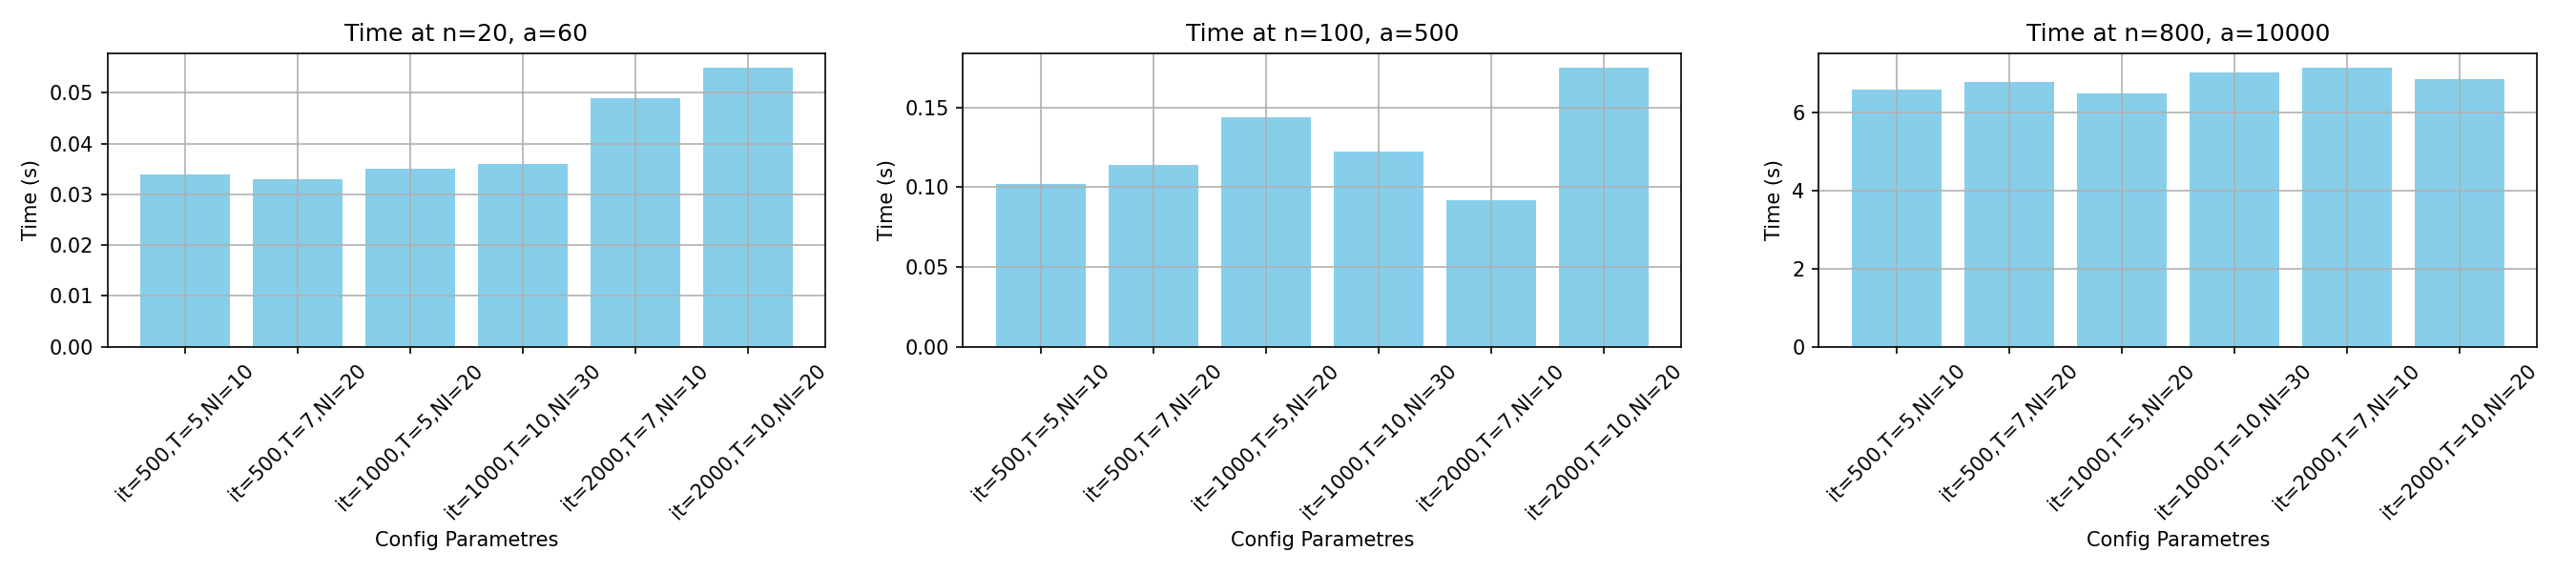
\includegraphics[width=1\textwidth]{img/scalability_plot.png} % Esempio di plot
\caption{Tempo di esecuzione medio in funzione del numero di nodi, configurazione \emph{maxIterations}, \emph{tabuTenure}, \emph{maxNoImprovement}.}
\label{fig:scalability}
\end{figure}

Una eventuale \emph{long-term memory}, basata sul conteggio di frequenza con cui i nodi appaiono o spariscono dal cover, potrebbe migliorare ulteriormente la diversificazione su istanze molto grandi, sebbene ciò comporti una maggiore complessità implementativa. Nel prossimo capitolo (\ref{sec:Conclusioni}) verranno esposti alcuni spunti di sviluppo e riflessioni conclusive sull'algoritmo e le sue prospettive future.

% Fine capitolo Risultati
